% !TeX root = RJwrapper.tex
\title{Priority Elastic Net: A Hierarchical Framework for Heterogeneous Data Integration}
\author{by L Musib, by H. Mouriño, by E. Carrasquinha}

\maketitle

\abstract{
The rapid development of high-throughput technologies has produced increasingly complex and high-dimensional biological datasets, requiring advanced statistical methods. In such contexts, where the number of variables exceeds the number of observations, variable selection is crucial to improve prediction accuracy, reduce variance, and enhance interpretability. The integration of multiple omics datasets collected from the same set of patients introduces additional challenges, including heterogeneity, multicollinearity, and the need to prioritise information across data blocks. The Priority Elastic Net method addresses these challenges by incorporating prior knowledge of block structure. The priorityelasticnet package, available on CRAN, provides implementations for continuous, binary, multinomial, and survival outcomes in R. It sequentially fits elastic net (or adaptive elastic net) models to predefined blocks, enabling customised penalisation and flexible feature selection. This framework is particularly useful for multi-omics integration and other structured high-dimensional applications.
}

\hypertarget{Introduction}{%
\section{Introduction}\label{sec:intro}}

In the field of high-dimensional omics data analysis, regularisation techniques have become essential due to their ability to simultaneously select variables and estimate models, particularly when the number of explanatory variables greatly exceeds the sample size. A variety of computational packages have been developed to implement these techniques effectively, addressing a range of research needs in omics studies.

The least absolute shrinkage and selection operator (lasso) \citep{tibshirani1996regression} is a popular method for regression that uses an $\ell_1$ penalty to
achieve a sparse solution.
This idea has been broadly applied, for example, to generalized linear models \citep{tibshirani1996regression} and Cox proportional hazard models for survival data.
\citep{tibshirani1997lasso}.

While the lasso excels at promoting sparsity, it does not account for feature ordering or structure, a limitation particularly pronounced in high-dimensional omics data. To overcome this, extensions such as the fused lasso \citep{Tibshiranifusedlasso} incorporate penalties that encourage smoothness along ordered features. In contrast, the adaptive lasso \citep{Zouadaptivelasso} dynamically adjusts penalties to improve variable selection. These methods are integrated into specialised packages, such as \CRANpkg{SQOPT} \citep{arnold2022package} and \CRANpkg{adalasso}.

Despite its success in many applications, the lasso method struggles with variable selection when features are highly correlated, as it tends to select only one variable from a group, a limitation in applications such as microarray data analysis, where genes often interact in networks. To address this issue, \cite{Zou2005elasticnet} proposed the elastic net penalty, which is a weighted sum of the $\ell_1$ norm and the square of the $\ell_2$ norm of the coefficient vector $\bm{\beta}$.
The first term enforces the sparsity of the solution, whereas the second term encourages a more balanced selection of correlated variables.

The \CRANpkg{glmnet} package, one of the most popular implementations in R and Python, provides a robust, widely used framework for applying lasso, elastic net, and related techniques.
 Details may be found in \cite{friedman2010regularization},  \cite{simon2011regularization},
 \cite{tibshirani2012strong}. The \CRANpkg{glmnet} R package \citep{friedman2010regularization} contains efficient functions for computing the elastic net solution for a complete path-wise optimisation. The minimisation problems are solved via cyclic coordinate descent \citep{van2007prediction}, with the core routines programmed in Fortran for computational efficiency. Earlier versions of the package contained specialised Fortran subroutines for a handful of popular GLMs and the Cox model for right-censored survival data. The package includes functions for performing K-fold cross-validation (CV) for hyperparameter optimisation, plotting coefficient paths and CV errors, and predicting on future data. The package can also accept the predictor matrix in sparse matrix format: this is especially useful in certain applications where the predictor matrix is both large and sparse. In particular, this means that we can fit unpenalised GLMs with sparse design matrices, something that the \CRANpkg{glm} function
from the package \CRANpkg{stats} does not support.

Version 4.0 and later of \CRANpkg{glmnet} \citep{friedman2023glmnet} represent a significant release that expands the package's capabilities for survival modelling. It supports multiple events per subject, delayed entry, time-dependent covariates and/or strata, and other extensions, through the (start, stop] formulation of the survival data that specifies the start and end of each time interval. Additionally, it includes sparse $X$ inputs, and the much-requested \texttt{survival:survfit} method. The package computes the elastic net regularisation path for all GLMs, Cox models with (start, stop] data and strata, and includes a simplified implementation of the relaxed lasso \citep{hastie2020best}, providing greater flexibility for high-dimensional data analysis.

To address the instability often observed in methods based on the elastic net, adaptive strategies have been incorporated into regularisation frameworks. One such approach is the Adaptive Elastic Net (AENet), implemented in the R package \CRANpkg{msaenet}. AENet refines the elastic net regularisation method to enhance feature selection and model performance, particularly in high-dimensional settings or in the presence of multicollinearity among predictors. Unlike the standard elastic net, which applies the same penalty to all coefficients, AENet introduces adaptive weighting to penalise features differently based on their importance \citep{zou2009adaptive}.

In the era of multi-omics research, integrating data across multiple omics layers is crucial for harnessing the complementary information from diverse biological systems. Single-data-type models often fail to capture the full complexity of underlying biological processes. Recent advances have underscored the importance of combining high-dimensional omics data, including clinical information, gene expression, methylation profiles, and other omics layers, to improve predictive modelling frameworks \citep{huang2017more}.

Using multi-omics data in prediction models is promising because each omics type offers unique and valuable information for predicting phenotypic outcomes.  However, effectively integrating various types of omics data presents several challenges. First, there is an overlap in the predictive information each data type provides. Second, the levels of predictive details differ between the 'blocks' of variables (which can correspond to the type of data, e.g., the block of clinical variables or the block of gene expression variables) and depend on the particular outcome considered \citep{QingZhaoCombinmultidimensional}. Third, the interactions between variables of different data types must be considered \citep{huang2017more}. In recent years, different methods have been proposed to address this topic. \cite{Simonsparse-group} presented the sparse group lasso, a prediction method for grouped covariate data that automatically removes non-informative covariate groups and performs lasso-type variable selection for the remaining covariate groups. The \CRANpkg{SGL} package \citep{simon2018package} in R is a notable implementation that combines the strengths of group lasso and lasso for sparse solutions at both the group and individual variable levels.

One limitation of using sparse lasso in multi-omics data applications is that it does not adequately account for the varying levels of predictive information across different data blocks.  In contrast, the IPF-LASSO \citep{BoulesteixIPF-LASSO}, a lasso-type regression method for multi-omics data, addresses this by assigning individual penalty parameters to different omics data types, allowing incorporation of prior biological knowledge or practical constraints. One common issue for all variations of LASSO, including IPF-LASSO, is instability. Even small modifications to the dataset can significantly change the selected model. The IPF-LASSO method addresses the unique challenges of multi-omics data integration, particularly the differing levels of predictive information across data blocks. The \CRANpkg{ipflasso} package \citep{boulesteix2015ipflasso} has been developed to implement this method, offering a tailored approach to multi-omics data analysis.

Building on the idea of representing each omics dataset as a block, \cite{Klau2018prioritylasso} introduced the Priority-Lasso method, implemented in the \CRANpkg{prioritylasso} package, as a lasso-based approach designed explicitly for multi-omics data analysis. This method emphasises practical usability by allowing users to assign priority rankings to data blocks based on cost or relevance.

The package \CRANpkg{prioritylasso}, developed for applications involving continuous, binary, and survival outcomes, was initially released on CRAN as version 0.2.4, as documented in \cite{klau2017prioritylasso}. Available from the CRAN repository, the package builds on the lasso regression implementation in \CRANpkg{glmnet} \citep{friedman2010regularization}. The Cox-Lasso model employs the regularisation method described by \cite{simon2011regularization}. In version 0.3.1, functionality was added to address blockwise missing data. This means that for some observations, not all blocks are observed. To address this type of missingness, \CRANpkg{prioritylasso} offers several options for fitting a model in datasets with missing values. Nevertheless, priority-lasso struggles with multicollinearity, often arbitrarily selecting one variable from correlated groups while excluding others, resulting in unstable models. This approach applies block prioritisation to manage overlapping predictive information, ensuring that lower-priority blocks are not excluded but adjusted for previously explained variance.
Although Priority-Lasso effectively promotes sparsity, it may lack stability, particularly in datasets with highly correlated variables or variable groupings of varying sizes. Furthermore, its sequential prioritisation framework does not fully exploit the hierarchical or grouped structures common in omics data, potentially limiting its applicability.

To address some of the limitations highlighted in the literature and summarised above, the Priority Elastic net method was proposed by \cite{musib2024priority} as an enhancement of the Priority-Lasso approach introduced by \cite{Klau2018prioritylasso}. By integrating the elastic net penalty, which balances $\ell_1$ and $\ell_2$ regularisation, Priority Elastic Net effectively mitigates issues related to multicollinearity and model instability. This method enhances the retention of predictive features from lower-priority blocks, providing greater flexibility for handling complex, high-dimensional datasets.

The \CRANpkg{priorityelasticnet} package \citep{musib2025priorityelasticnet} is available on the Comprehensive R Archive Network (CRAN) at \url{http://CRAN.R-project.org/package=priorityelasticnet}.

\hypertarget{Priority elastic net}{%
\section{Priority elastic net} \label{sec:models}}
A growing number of studies have utilised multi-omics data for various precision medicine-related machine learning tasks, including disease diagnosis, patient sub-phenotyping, and predicting disease or mortality risk. However, data from different omics modalities can be heterogeneous and noisy, with various underlying distributions and scales \citep{huang2017more}. Thus, the way these data are integrated significantly impacts subsequent analyses and interpretations.

The Priority Elastic Net \citep{musib2025priorityelasticnet} builds upon the Priority-Lasso framework \citep{Klau2018prioritylasso}, incorporating elastic net principles to address limitations in handling highly correlated predictors. The implementation of the \CRANpkg{priorityelasticnet} package adapts several functions from the \CRANpkg{prioritylasso} package \citep{Klau2018prioritylasso,klau2017prioritylasso}. While Priority-Lasso introduced a hierarchical structure to effectively integrate multi-omics data into regression models, it struggles with datasets containing strongly correlated variables. By combining the strengths of \(\ell_1\) and \(\ell_2\) regularisation \citep{Zou2005elasticnet}, the Priority Elastic Net promotes a grouping effect, ensuring that correlated predictors are retained within the model. This enhancement enables the Priority Elastic Net to deliver improved robustness, interpretability, and accuracy, making it particularly suited to high-dimensional and complex omics datasets.

In the following subsections, we outline the theoretical foundations and computational implementation of Priority Elastic Net optimisation across Gaussian, multinomial, binomial, and Cox regression frameworks, demonstrating its potential in enhancing variable selection. We introduce the main functions of the \CRANpkg{priorityelasticnet} package, which address essential data characteristics, such as handling missing values, and include cross-validation methods. Illustrative examples, primarily based on the Gaussian distribution, are provided to demonstrate their usage. Finally, we introduce the Priority-Adaptive Elastic Net, which further improves model performance by dynamically adjusting variable priorities during optimisation.

\subsection{Priority elastic net for a gaussian family}\label{sub:Gaussian}

We consider the standard setup for linear regression, where the response variable \( Y \in \mathbb{R} \) is continuous. Let \(x_{ij}\) be the independent variable \(j\) of individual \(i\), where \(i = 1, \ldots, n\) , \(j = 1, \ldots, p\)  with \(n\) being the total number of individuals and \(p\) the number of independent variables.  The vector \(\bm{x}_i = (x_{i1}, x_{i2}, \ldots, x_{ip})^T\) represents the set of independent variables for the individual \(i\).
For simplicity, the predictor variables \( x_{ij} \) are transformed to z-scores.

In high-dimensional settings, where the number of predictors $(p)$ may exceed the number of observations $(n)$, or where the predictors exhibit strong correlations, traditional linear regression methods often struggle. Issues such as overfitting and multicollinearity reduce the reliability and interpretability of the estimated regression coefficients. To address these challenges, regularisation methods, such as the elastic net, have been developed. The standard elastic net method \citep{Zou2005elasticnet} estimates the regression coefficients $\beta_{1}, \ldots ,\beta_{p} $ associated with the $p$ regressors by minimizing the expression:

 \begin{equation}
 \label{eq: elastic net}
\hat{\bm{\beta}}_{EN}=\arg \min_{\bm{\beta}} \Bigg[ \frac{1}{n}\sum\limits_{i=1}^{n}\bigg(y_i- \beta_{0}- \sum\limits_{j=1}^{p}x_{ij}\beta_j\bigg)^2 +\lambda\sum_{j=1}^p \left(\alpha |\beta_j| + \frac{(1 - \alpha)}{2}  \beta_j^2\right)\Bigg], 
 \end{equation}

\noindent where \(\lambda \geq 0\) is a tuning parameter, and \(\alpha \in [0, 1]\) is a higher-level hyperparameter that controls the balance between the lasso and ridge penalties.
A sequence of models is typically fitted across a range of 
\(\lambda\) values, while the value of  \(\alpha\)
 is predetermined based on the desired characteristics of the prediction model. For example, ridge regression \citep{Hoerl1970ridge} is defined with \(\alpha = 0\), while lasso regression \citep{tibshirani1996regression} is defined with \(\alpha = 1\). 

The final value of \(\lambda\) is usually chosen via cross-validation: we select the coefficients corresponding to the \(\lambda\) value that minimises the cross-validated error as the final model.

Coordinate descent solves the optimisation problem by iteratively optimising each coefficient \(\beta_j\)
 while keeping the others fixed \citep{friedman2010regularization}. 
 The formula for updating \(\beta_j\) is given by:\\
\[
\hat{\beta}_j = S\left(\frac{1}{n} \sum_{i=1}^n x_{ij} \left( y_i - \hat{y}_i^{(j)} \right), \lambda \alpha \right)  \frac{1}{1 + \lambda (1 - \alpha)},
\]
where
\[
\hat{y}_i^{(j)} = \hat{\beta}_0 + \sum_{\ell \neq j} x_{i\ell} \hat{\beta}_\ell,
\]
and the soft-thresholding operator \(S(z, \gamma)\) is defined as:
\[
S(z, \gamma) = \text{sign}(z) \max(|z| - \gamma, 0).
\]
In this context, the notation is adapted to address the case of grouped variables, as considered in this work. The model partitions the predictors into $B$ blocks, with the observations of the $p_{b}$ variables from block $b$ for subject $i$ being represented as $ (x_{i1}^{(b)}, . . . , x_{ip_{b}}^{(b)} )$, for $i=1,...,n$ and for $b = 1, . . . , B$. 
This block structure reflects the natural organisation of multi-omics data, where each omics layer (e.g., transcriptomics, proteomics, methylation) typically forms a separate block, often combined with a clinical block. More generally, it can also represent other meaningful groupings, such as biological pathways or categories of clinical variables. Just as \( x^{(b)}_{ij} \) is defined, \( \beta^{(b)}_{j} \) is the regression coefficient of the \( j^{th} \) variable from  block $b$, with \( j \) ranging from 1 to \( p_b \). Accordingly, \( \hat{\beta}^{(b)}_{j} \) denotes the respective estimated value.

Consider \(\bm{\pi} = (\pi_1, \ldots, \pi_B)\) as a reordering of the sequence \((1, \ldots, B)\), signifying the priority order of blocks, where \(\pi_1\) represents the index of the block with highest significance and \(\pi_B\) denotes the one of least priority. Subsequently, a hierarchical method is employed to construct the predictive model, adhering to this established order of block importance. The first step is to estimate the $\beta_j^{(\pi_1)}$ coefficients, by minimising:
 \begin{equation}
 \label{eq:elstic_block1}
 l(\bm{\beta}^{(\pi_1)}) = \sum\limits_{i=1}^{n}\bigg(y_i- \beta_0^{(\pi_1)}-\sum\limits_{j=1}^{p_{\pi_1}}x_{ij}^{(\pi_1)}\beta_j^{(\pi_1)}\bigg)^2 + \lambda^{(\pi_1)} \sum\limits_{j=1}^{p_{\pi_1}} \Big( \alpha \lvert \beta_j^{(\pi_1)} \rvert + \frac{(1 - \alpha)}{2}(\beta_j^{(\pi_1)})^2 \Big).  
\end{equation}
The fitted linear predictor, $\hat{\eta}_{1,i}(\bm{\pi})$, in this step is given as:
\begin{equation}
\hat{\eta}_{1,i}(\bm{\pi})= 
\hat{\beta}^{(\pi_1)}_0+
\hat{\beta}_1^{(\pi_1)}x_{i1}^{(\pi_1)} + . . . + \hat{\beta}_{p_{\pi_1}}^{(\pi_1)} 
x_{ip_{\pi_1}}^{(\pi_1)}.
\end{equation}
Next, the elastic net method is applied to the block of predictors with the second highest priority, incorporating the fitted linear predictor from the first step as an offset. The goal is to determine the values of $\hat{\beta}_{1}^{(\pi_2)}, \ldots, \hat{\beta}_{p_{\pi_2}}^{(\pi_2)},$ which are the coefficients corresponding to the predictors within the second priority block, $\pi_2$. These coefficients are determined by minimising a specific criterion, outlined as follows:
\begin{equation}
 l(\bm{\beta}^{(\pi_2)}) = \sum\limits_{i=1}^{n}\bigg(y_i- \hat{\eta}_{1,i}(\bm{\pi})-\beta_0^{(\pi_2)}-\sum\limits_{j=1}^{p_{\pi_2}}x_{ij}^{(\pi_2)}\beta_j^{(\pi_2)}\bigg)^2 + \lambda^{(\pi_2)} \sum\limits_{j=1}^{p_{\pi_2}} \Big( \alpha \lvert \beta_j^{(\pi_2)} \rvert + \frac{(1 - \alpha)}{2}(\beta_j^{(\pi_2)})^2 \Bigg\}. 
\end{equation}

The linear predictor for the second step,
\(\hat{\eta}_{2,i}(\bm{\pi})\), is derived by adding the offset obtained from the first step, 
\(\hat{\eta}_{1,i}(\bm{\pi})\), with the linear combination of the predictors in the second priority block and their respective estimated coefficients,
\(\hat{\beta}^{(\pi_2)}\). This relationship can be represented as:

\begin{equation}
\hat{\eta}_{2,i}(\bm{\pi}) =\hat{\eta}_{1,i}(\bm{\pi}) + 
\hat{\beta}_0^{(\pi_2)}+
\hat{\beta}_1^{(\pi_2)}x_{i1}^{(\pi_2)} + . . . + \hat{\beta}_{p_{\pi_2}}^{(\pi_2)}x_{ip_{\pi_2}}^{(\pi_2)}.
\end{equation}

Then, similarly, the model is fitted to the block with the third highest
priority, using the linear score from the second step as an offset. All remaining
blocks are treated in the same manner, 
\begin{equation}
\hat{\eta}_{b,i}(\bm{\pi}) = \hat{\eta}_{b-1,i}(\bm{\pi}) + 
\hat{\beta}_0^{(\pi_b)}+
\hat{\beta}_{ 1}^{(\pi_b)} x_{i1}^{(\pi_b)} + \ldots + \hat{\beta}_{ p_{\pi_b}}^{(\pi_b)} x_{ip_{\pi_b}}^{(\pi_b)},
\end{equation}
where $\hat{\eta}_{0,i}(\bm{\pi}) = 0$ and $b = 1, \ldots, B$.

The fitting procedure is carried out sequentially through the blocks up to $\pi_B$, yielding the set of coefficient estimates $\hat{\beta}^{(\pi_b)}$ for $b = 1, \ldots, B$. The final fitted linear predictor becomes
\begin{equation}
\hat{\eta}_{i}(\bm{\pi}) = 
\sum_{b=1}^{B} 
  \hat{\beta}_0^{(\pi_b)}+
\sum_{b=1}^{B} \sum_{j=1}^{p_{\pi_b}} \hat{\beta}^{(\pi_b)}_j x^{(\pi_b)}_{ij}.
\end{equation}

As previously discussed, Priority Elastic Net assigns a priority order to blocks, allowing the model to incorporate prior knowledge. However, this hierarchical structure may negatively affect predictive accuracy by underestimating the influence of predictors in lower-priority blocks and potentially discarding informative variables. This issue occurs because the linear score in each block, \(\hat{\eta}_{b,i}(\bm{\pi})\), tends to overfit the contribution of predictors in the \(b\)-th block to the response \(y_i\). Specifically, the estimation of $\hat{\eta}_{b,i}(\bm{\pi})$ tends to overfit the effects of predictors in the $b$-th block on the response $y_i$. This overfitting arises because the coefficients $\hat{\beta}_1^{(\pi_b)}, \ldots, \hat{\beta}_{p\pi_b}^{(\pi_b)}$ are estimated using data that includes $y_i$, the response being predicted. Consequently, the overfitted score $\hat{\eta}_{b,i}(\bm{\pi})$ captures variability in $y_i$ that might better be explained by predictors in subsequent blocks. When this overfitted estimate is used as an offset, it limits lower-priority blocks' ability to account for unexplained variability in $y_i$, thereby undermining the model's overall predictive accuracy.

To mitigate this overfitting problem, cross-validated offsets, $\hat{\eta}_{b,i}(\pi)_\text{CV}$, previously introduced in the Priority Lasso framework, are also applied in the Priority Elastic Net to improve generalisation. In this approach, a dataset \(S\) is partitioned using \(K\)-fold cross-validation, and the cross-validated offsets are determined to effectively address the identified overfitting issues. The cross-validated offsets are computed iteratively as follows:
    \begin{equation}
        \hat{\eta}_{b,i}(\bm{\pi})_\text{CV} = \hat{\eta}_{b-1,i}(\bm{\pi})_\text{CV} +
        \hat{\beta}^{(\pi_b)}_{S \setminus S_{k,0}}
        + \hat{\beta}^{(\pi_b)}_{S \setminus S_{k,1}}x_{i1}^{(\pi_b)}
        + \ldots 
        + \hat{\beta}^{(\pi_b)}_{S \setminus S_{k,p_{\pi_b}}}x_{ip_{\pi_b}}^{(\pi_b)},  \, \, \,  b = 1, . . . , B   
    \end{equation}
where the process starts with the initial condition: \,\,\,\, $\hat{\eta}_{0,i}(\bm{\pi})_\text{CV} = 0$.

Priority Elastic Net is implemented in the \CRANpkg{priorityelasticnet} function in our R package of the same name. This function includes the option \code{cvoffset}, which allows users to choose between cross-validated offsets and standard offsets estimated without cross-validation, as outlined in the algorithm presented in this section.

To illustrate the implementation of Priority Elastic Net for the Gaussian family, a synthetic dataset was simulated to mimic the high-dimensional characteristics typical of multi-omics studies. In this example, \(n=100\) observations and \(p=500\) predictors are generated, with only the first 10 predictors contributing to the response variable.
{\small
\begin{verbatim}
set.seed(123)
n <- 100  
p <- 500  
X <- matrix(rnorm(n * p), n, p)
beta <- rnorm(10) 
Y <- X[, 1:10] %*% beta + rnorm(n)
\end{verbatim}
}
Before applying Priority Elastic Net, the user must first specify a block structure for the covariates, where each covariate belongs to exactly one of the \( B \) blocks, and second, a priority order for these blocks. In this framework, three blocks of continuous predictor variables were analysed, all of which are subject to penalisation, while adapting our notation to account for variables forming groups as considered in this work. The first entry in the \code{blocks} list specifies the indices of the variables that belong to the block assigned the highest priority (priority 1), which is the first block included in the model. As an example, if \code{blocks = list(1:10, 11:30, 31:500)}, the first priority block contains the first 10 variables in the data matrix. Similarly, the block assigned priority 2 includes variables 11-30, whereas the block assigned priority 3 comprises variables 31-500.
{\small
\begin{verbatim}
    blocks <- list(block1 = 1:10, block2 = 11:30, block3 = 31:500)
\end{verbatim}
}
The \code{priorityelasticnet} function fits a hierarchical elastic net model across multiple blocks of variables. In this example, the model is fitted with \code{family="gaussian"} for continuous response variables, with the \code{block1.penalization} parameter controlling how the first block (priority 1) is treated during model fitting.
{\small
\begin{lstlisting}
fit_gaussian <- priorityelasticnet(
  X = X, Y = Y, family = "gaussian", blocks = blocks,
  block1.penalization = TRUE, standardize = TRUE,
  lambda.type = "lambda.min", max.coef = c(Inf, Inf, Inf),
  nfolds = 10, type.measure = "mse", alpha = 0.6,
  cvoffset = TRUE, cvoffsetnfolds = 10,
  adaptive = FALSE, initial_global_weight = FALSE
)
\end{lstlisting}
}
When \code{block1.penalization = TRUE}, the function applies a standard elastic net model to the first block, treating it similarly to other blocks. The predictions from this first block are then used as offsets in the elastic net fitting of the subsequent blocks, following their priority order. Conversely, when \code{block1.penalization = FALSE}, the function fits the first block without penalisation, making this setting appropriate for scenarios where clinical predictors (with $p<n$) are included. Clinical predictors in the first block are not penalised to preserve their established relevance. In this case, the unpenalized predictions serve as offsets for the subsequent elastic net fits for lower-priority blocks.

The \code{standardize = TRUE} leads to a standardisation of the predictor variables. In case of an unpenalized first block, the predictor variables for the first block are not standardised. Please note that the returned coefficients are rescaled to the original scale of the predictor variables as provided in $\mathbf{X}$. Therefore, new data in \code{predict.priorityelasticnet} should be on the same scale as $\mathbf{X}$.

The \code{nfolds} and \code{lambda.type} are options referring to the cross-validation procedure in \code{cv.glmnet}. The \code{nfolds} specifies the number of folds in the procedure, while \code{lambda.type} handles the amount of cross-validation error. It can be set to either \code{lambda.min}, which is also the default, or \code{lambda.1se}. The \code{lambda.min} gives the result with minimum mean cross-validation error, whereas \code{lambda.1se} gives the result such that the cross-validation error is within one standard error of the minimum, and thus leads to more sparse results. Note that the latter can only be chosen in combination with no restrictions in \code{max.coef}.

The function used for every Priority Elastic net fit is \CRANpkg{glmnet}, which creates a sequence of lambda values. The lambda which is chosen according to \code{lambda.type} is the lambda on position \code{lambda.ind} of the sequence and its value is stored in \code{lambda.min}. In general, the lower the value of \code{lambda.ind}, the higher the \code{lambda.min} and thus the penalisation. This leads to more sparse models. The number of lambda values can be chosen with an optional argument. 

The values of lambda are automatically generated in each call of \CRANpkg{glmnet}, based on the input data and model parameters, and may therefore differ between runs. Consequently, $\lambda$ values from separate model fits cannot be directly compared unless a common sequence is explicitly defined. The corresponding mean cross-validated error is stored in the list \code{min.cvm}. The interpretation of its values depends on the argument \code{type.measure}.

The \code{type.measure} is the accuracy/error measure computed in cross-validation. It should be "class" (classification error) or "auc" (area under the ROC curve) if \code{family="binomial"}, "mse" (mean squared error) if \code{family="gaussian"} and "deviance" if \code{family="cox"}, which uses the partial-likelihood.

The \code{cvoffset} parameter is a logical flag that determines whether cross-validation (CV) should be used to estimate offsets during elastic net fitting. By default, its value is set to FALSE, meaning no CV is performed for offset estimation unless explicitly specified. If \code{cvoffset} is set to TRUE, the \code{cvoffsetnfolds} parameter becomes relevant, allowing the user to specify the number of folds for the CV procedure used in estimating the offsets. The default value for \code{cvoffsetnfolds} is 10, which means the data will be split into 10 folds during the CV process.

The \texttt{adaptive} argument in \CRANpkg{priorityelasticnet} introduces an advanced layer of flexibility by enabling the adaptive elastic net, which enhances the standard elastic net through the use of data-driven adaptive weights. This methodology is explained in detail in Section \ref{subsec:PAD-E}. Additionally, the \texttt{initial\_global\_weight} option allows for further customisation by enabling users to apply a global weight across all predictors before fitting the adaptive elastic net. This argument is also discussed in detail in Section~\ref{subsec:PAD-E}.

The main results of the fitted model from the \CRANpkg{priorityelasticnet} are stored in an object returned by the functions provided by the package, which includes the coefficient estimates, tuning parameters, and related outputs. The estimated model parameters can be extracted using the \texttt{coef.priorityelasticnet} function, a method of the generic \texttt{coef()} function specifically designed to retrieve the coefficients from the fitted model object. It represents the relationship between the predictors and the response variable. Understanding these coefficients is essential for gaining insights into how each predictor influences the outcome, particularly in the context of penalised regression models where some coefficients may be shrunk towards zero or set to zero due to regularisation.

The \CRANpkg{priorityelasticnet} package was developed under the assumption that practitioners have prior knowledge of the data, enabling them to specify the priorities. However, it may be that, especially in the presence of several blocks, it is not clear which block order is best. For this reason, \texttt{cvm\_priorityelasticnet} was implemented. This function allows the user to define multiple possible lists of blocks. The function selects the optimal block order based on the mean cross-validated error. Similarly, several vectors with maximal coefficients can be specified in \texttt{max.coef.list}. The following example demonstrates how to use the \texttt{cvm priorityelasticnet} function to evaluate and compare different block configurations. 
{\small
\begin{lstlisting}
fit_cvm <- cvm_priorityelasticnet(
  X = X, Y = Y, weights = rep(1, n),
  foldid = sample(rep(1:10, length.out = n)),
  family = "gaussian", type.measure = "mse",
  blocks.list = list(list(bp1 = 1:10, bp2 = 11:30, bp3 = 31:500),
                list(bp1 = 1:10, bp2 = 31:500, bp3 = 11:30)),
  max.coef.list = list(c(Inf, Inf, Inf), c(Inf, 100, Inf)),
  block1.penalization = TRUE,
  lambda.type = "lambda.min",
  standardize = TRUE,
  nfolds = 10,
  cvoffset = TRUE,
  cvoffsetnfolds = 10,
  alpha = 0.6,
  adaptive = FALSE,
  initial_global_weight = FALSE)
\end{lstlisting}
}
In this example, two distinct block configurations, \code{blocks.list}, are defined and passed to the \code{cvm\_priorityelasticnet} function. This function performs cross-validation on each configuration, calculating the mean squared error (MSE) for each model. Comparing these MSE values enables the identification of the block configuration that yields the best predictive performance.
The output from \code{fit\_cvm} provides detailed information regarding the performance of each block configuration, including cross-validated MSE values, the optimal lambda for each configuration, and the number of non-zero coefficients selected by the model. The elements contained in the R object \code{fit\_cvm} can be summarised as follows:
\begin{itemize}
\item \texttt{fit\_cvm\$best.blocks}: provides the block configuration that achieves the best cross-validated performance in terms of MSE;

\item \texttt{fit\_cvm\$best.blocks.indices}: provides the position (index) of the block configuration that achieves the best cross-validated result;

\item \texttt{fit\_cvm\$best.max.coef}: provides the blockwise maximum number of non-zero coefficients allowed in the selected optimal configuration.

\end{itemize}

Handling missing data is crucial for constructing robust models, particularly when working with real-world datasets that include missing values. The \CRANpkg{priorityelasticnet} package provides several options for handling missing data, allowing users to select the most suitable strategy based on the dataset's characteristics and analysis goals.

The \code{mcontrol} argument in \CRANpkg{priorityelasticnet} allows for specifying how missing data should be handled. This flexibility ensures the model can be effectively fitted, even with incomplete data, which might otherwise result in biased estimates or diminished predictive power.

The \CRANpkg{priorityelasticnet} package provides methods to handle blockwise missing data, which can be specified through the \code{mcontrol} argument using the \code{missing.control()} function: 
{\small
\begin{lstlisting}
missing.control(handle.missingdata = c("none", "ignore", "impute.offset"),
  offset.firstblock = c("zero", "intercept"),
  impute.offset.cases = c("complete.cases", "available.cases"),
  nfolds.imputation = 10,
  lambda.imputation = c("lambda.min", "lambda.1se"),
  perc.comp.cases.warning = 0.3,
  threshold.available.cases = 30,
  select.available.cases = c("maximise.blocks", "max"))
\end{lstlisting}
}
\code{handle.missingdata}: how blockwise missing data should be treated. The default is "none", meaning that no action is taken and missing values remain as provided, "ignore" ignores the observations with missing data for the current block, "impute.offset" imputes the offset for the missing values.

When \code{handle.missingdata="ignore"}, the elastic net is fitted to each block using only the observations without missing values in that block. This approach avoids data imputation and ensures all available data is utilised. However, for observations with missing values in the current block, no offset can be computed for the next block. 
To address this issue, the following strategies are implemented:
\begin{itemize}
    \item If observations are missing in the current block, the offset (including the intercept) from the previous block is carried forward.
    \item If observations are missing in the first block, 
     the offset for the second block is set either to \(0\) or to the estimated intercept of the first block.
\end{itemize}

The offset of a block \(b\) for an observation \(i\) is denoted as \(\delta_{b,i}\), and is formally defined as:
\[
\delta_{1,i} =
\begin{cases} 
    0 & \text{if } x^{(1)}_{i1}, \dots, x^{(1)}_{ip_1} \text{ are missing} \\
    \hat{\eta}_{1,i} \text{ or } \hat{\beta}^{(1)}_0 & \text{if } x^{(1)}_{i1}, \dots, x^{(1)}_{ip_1} \text{ are not missing}
\end{cases}  \quad \quad \quad \quad \quad \quad \quad \quad \ \
\]
\[
\delta_{b,i} =
\begin{cases} 
    \delta_{b-1,i} & \text{if } x^{(b-1)}_{i1}, \dots, x^{(b-1)}_{ip_{b-1}} \text{are missing}\\
    \hat{\eta}_{b-1,i} & \text{if } x^{(b-1)}_{i1}, \dots, x^{(b-1)}_{ip_{b-1}} \text{are not missing}
\end{cases}, \quad \text{for} \ b = 3, \dots, B,
\] 

\noindent where \(\hat{\eta}_{b,i}\) is the prediction from block \(b\) for the \(i\)-th observation.
\code{offset.firstblock}:
determines if the offset of the first block for missing observations is zero or the intercept of the observed values for \code{handle.missingdata = "ignore"}.

For \code{handle.missingdata="impute.offset"}, it is similar to the previous method; the elastic net models applied to the individual blocks utilise only the available data, and no covariates are imputed. However, unlike the previous approach, the offset for observations with missing values is not retained from the earlier block; instead, it is imputed. This approach offers the benefit of imputing only a single value, rather than potentially a very large number of covariates. The concept behind this method is inspired by \citet{hieke2016integrating}, which only imputes an offset. In their work, they utilise just three blocks, resulting in a fixed configuration for the imputation model. Here, we extend this idea into a generalised framework, introducing two distinct strategies for selecting which blocks to use.
As Priority Elastic Net is an elastic net-based method, the imputation model uses an elastic net as well. Generally, any model that can predict a continuous outcome can be used as the imputation model. In the following sections, this is represented by only referencing a general regression model $F(\cdot)$. Let $F(\cdot)$ be a general regression model that can be trained by providing the dependent variable
and the independent variables.

The argument \code{impute.offset.cases} defines which observations are used to construct the imputation model for missing offsets. Supported options are \code{complete.cases}, which limits the imputation to fully observed cases (with the additional constraint that each observation may contain at most one missing block), and \code{all.available.cases}, which uses all observations for which data are available in the current block.

The first approach (\code{impute.offset.cases="complete.cases"}) utilises all blocks except the current one to impute the offset derived from the current block. For this method to work, the dataset must include some observations without missing values (complete cases). A reasonable lower limit for the number of complete cases must be established. Based on the work of \citet{hieke2016integrating}, who used 26 complete cases, the default threshold is set to 30 cases. Another limitation of this approach is that each observation with missing data can have at most one missing block, as all other blocks are required for the imputation model. A more formal description is provided below.

If only the complete cases are used for the imputation model and \( I = \{1, \ldots, n\} \)
is the set of observation indices, the observations used for the imputation model are defined as:
\[
I_{\text{comp,imp}} = \{i \in I \mid x^{(b)}_{i1}, \ldots, x^{(b)}_{ip_b} \text{ are not missing } \forall b\},
\]
where \( x^{(b)}_{i1}, \ldots, x^{(b)}_{ip_b} \) are the covariates of the \( b \)-th block of the \( i \)-th observation. 
Let \( F(\cdot) \) be a general regression model that can be trained by providing the dependent variable and the independent variables. Then \( \tilde{F}(\cdot) \) represents a trained regression model that returns its prediction when provided with the independent variables.

The algorithm below describes how, for an observation \( j \) with a missing block \( b \), 
the corresponding linear predictor (offset) is imputed as \( \hat{\kappa}_{\text{comp},b,j} \).

\begin{enumerate}
    \item Identify the set of complete cases \( I_{\text{comp,imp}} \), as defined above.
    \item For all observations \( i \in I_{\text{comp,imp}} \), compute the offset (linear predictor) 
    for block \( b \), denoted by \( \hat{\kappa}_{\text{comp},b,i} \).
    \item Train the regression model \( \tilde{F}(\cdot) \) using the complete cases \( I_{\text{comp,imp}} \), 
    where the dependent variable is the offset \( \hat{\kappa}_{\text{comp},b,i} \), 
    and the covariates are the predictors from all other observed blocks, collectively denoted by \( x^{(-b)}_i \)
    (that is, all blocks except the one currently missing block \( b \)).
    \item For the observation \( j \) with missing block \( b \), 
    use the trained regression model \( \tilde{F}(\cdot) \) to predict the value of the missing 
    offset \( \hat{\kappa}_{\text{comp},b,j} \).
\end{enumerate}

The offset for a given observation \( i \) in block \( b \) is defined as:
\[
\delta_{1,i} = 0,
\]
\begin{equation*}
\delta_{b,i} =
\begin{cases} 
    \hat{\eta}_{b-1,i}, & \text{if } x^{(b-1)}_{i1}, \dots, x^{(b-1)}_{ip_{b-1}} \text{ are observed}, \\
    \hat{\kappa}_{\text{comp},b-1,i}, & \text{if } x^{(b-1)}_{i1}, \dots, x^{(b-1)}_{ip_{b-1}} \text{ are missing},
\end{cases}
\end{equation*}

\begin{equation*}
\text{for } b = 2, \dots, B, \quad \forall i \text{ such that each observation } i 
\text{ contains at most one missing block } b.
\end{equation*}

where:
\begin{itemize}
    \item \(\delta_{b,i}\) denotes the offset for block \( b \) and observation \( i \);
    \item \(\hat{\eta}_{b-1,i}\) is the prediction obtained from block \( b-1 \) for observation \( i \);
    \item \(\hat{\kappa}_{\text{comp},b-1,i}\) represents the predicted (compensatory) offset 
    used when predictors in block \( b-1 \) are missing.
\end{itemize}

The previous approach consistently relies on all other blocks to impute the offset for a missing block. However, in many datasets, there may be no observations with complete cases, or observations may have more than one block missing. To address these situations, a more adaptable method was developed (\code{impute.offset.cases="all.available.cases"}). This approach segments the observations into different subsets based on their missingness patterns. A missingness pattern indicates which specific combination of blocks is missing for a particular observation. For each unique pattern, a separate imputation model is constructed and fitted.
\[
\delta_{1,i} = 0
\]
\[
\delta_{b,i} =
\begin{cases} 
    \hat{\eta}_{b-1,i}, & \text{if } x^{(b-1)}_{i1}, \dots, x^{(b-1)}_{ip_{b-1}} \text{ are not missing}, \\
    \hat{\kappa}^{\text{comp}}_{b-1,i}, & \text{if } x^{(b-1)}_{i1}, \dots, x^{(b-1)}_{ip_{b-1}} \text{ are missing},
\end{cases}
\]
\[
\text{for } b = 2, \dots, B, \quad \forall i \quad \text{such that every observation } i \text{ misses at most 1 block } b.
\]

The remaining arguments of the \code{missing.control} function are described below:
\begin{itemize}
    \item \code{nfolds.imputation	}: nfolds for the glmnet of the imputation model;

    \item \code{lambda.imputation	}: which lambda-value should be used for predicting the imputed offsets in \code{cv.glmnet};

    \item \code{perc.comp.cases.warning}:	percentage of complete cases when a warning is issued of too few cases for the imputation model.

    \item \code{threshold.available.cases}: if the number of available cases for \code{impute.offset.cases = available.cases} is below this threshold, \code{priorityelasticnet} tries to reduce the number of blocks included in the imputation model to increase the number of observations used for imputation;

    \item \code{select.available.cases}: determines how the blocks which are used for the imputation model are selected when \code{impute.offset.cases = available.cases}. max selects the blocks that maximise the number of observations, \code{maximise.blocks} tries to include as many blocks as possible, starting with the highest-priority ones.
\end{itemize}

Below, we demonstrate how to configure the \code{mcontrol} argument to handle missing data by imputing offsets. 

In this example, the \code{handle.missingdata = "impute.offset"} option, which is part of the missing data handling mechanism, enables the \CRANpkg{priorityelasticnet} function to impute missing values using an offset approach. This method is particularly advantageous for handling sporadic missing data, as it allows the model to utilise all available information without discarding incomplete observations.
{\small
\begin{verbatim}
mcontrol <- missing.control(handle.missingdata = "impute.offset",nfolds.imputation = 10)

fit_missing <- priorityelasticnet(
  X, Y,
  family = "gaussian",
  type.measure = "mse",
  blocks = blocks,
  mcontrol = mcontrol)
\end{verbatim}
}
The output includes details on how the missing data was handled, the imputation models employed (if applicable), and the overall model fit. 

The \code{predict.priorityelasticnet} function is used to generate predictions from a fitted model. This function can produce different types of predictions depending on the specified type parameter, including linear predictors, fitted values, or class probabilities (for classification models). The \code{handle.missingtestdata} parameter manages missing values in test data, with options such as \code{"none"}, \code{"omit.prediction"}, \code{"set.zero"}, or \code{"impute.block"}. In the next section, each of these options is explained in detail, including their functionality and the scenarios in which they are most appropriate. The \code{include.allintercepts} parameter determines whether intercepts from all blocks are included in the prediction (\code{TRUE}) or only from the first block (\code{FALSE} by default). The \code{use.blocks} parameter allows customising the blocks used for prediction, defaulting to \code{"all"} but allowing specification of block numbers. Additional customisation can be achieved through further arguments, making the function versatile for various prediction scenarios, including handling missing data and tailoring block selection to specific needs.

\subsection{Priority elastic net for a multinomial logistic regression}\label{sub:multinomial}

Regularised multinomial logistic regression models are widely used in multi-class classification, particularly in high-dimensional data settings. They are instrumental in applications such as bioinformatics and cancer research, where sparsity and interpretability are critical. However, existing regularisation methods often fail to incorporate domain-specific priorities among predictors. To address this, the Priority Elastic Net method, initially developed for binary logistic regression \citep{musib2024priority}, is extended to multinomial logistic regression. 
This novel extension enables the classification of multiple classes by iteratively fitting blocks of predictors with specific priorities. Grounded in well-established logistic regression principles, the multinomial model reduces to standard logistic regression in the binary case ($K=2$), where the logit function models the probability of the first class relative to the second. By preserving the block-prioritised variable selection structure, this method provides a flexible and interpretable framework for multiclass problems, making it particularly suited for high-dimensional applications.

Let \(\mathbf{ X} \), the predictor matrix, be an \( n \times p \) matrix,  where \( \mathbf{x}_i = ( x_{i1}, x_{i2}, \dots, x_{ip} )^T \)
is the \( i \)th row of \( \mathbf{ X} \), i.e., the \( i \)th observation. The response vector \( \mathbf{Y} = ( Y_1, Y_2, \dots, Y_n )^T \) is an
\( n \times 1 \) vector, where the response \( Y_i \) is categorical, taking a value \( y_i \in \{1, 2, \dots, K\} \) for \( K \geq 3 \).
This concept has been effectively modelled in previous research, including the works of \citep{zhu2004classification} and \citep{friedman2010regularization}, with
\begin{equation}
P(Y_i = \ell \mid \mathbf{x}_i) = \frac{\exp \left(\beta_{0,\ell} + \mathbf{x}_i^T \boldsymbol{\beta}_{ \ell} \right)}{\sum_{k=1}^{K} 
\exp \left(\beta_{0,k} + \mathbf{x}_i^T\boldsymbol{\beta}_{k}\right)}, \quad \ell = 1, \dots, K,\,\,\,i=1,\ldots, n.
\end{equation}
where $\boldsymbol{\beta}_{\ell} = (\beta_{1\ell}, . . . , \beta_{p\ell})^T$ are coefficients estimated by minimizing the following negative log-likelihood function
for observations \( \{ (\mathbf{x}_i, y_i) \}_{i=1}^{n} \), where each \( y_i \) is encoded as \( \mathbf{y}_i = (y_{i1}, \dots, y_{iK})^T \) with \( y_{ik} = 1_{y_i = k} \):
\begin{equation}\label{regularizedmultinomial}
\ell(\boldsymbol{\beta}) = -\frac{1}{n} \sum_{i=1}^{n} \log P(Y_i = y_i \mid \mathbf{x}_i) + \lambda F_{\alpha}(\boldsymbol{\beta})
\end{equation}

\noindent where $\boldsymbol{\beta}$ denotes the matrix of dimension $(p + 1) \times K$, with the parameters $\beta_{0,\ell}$ and
$\boldsymbol{\beta}_{\ell}$ in its columns.

In Eq.~\eqref{regularizedmultinomial}, $y_{i}$ represents the observed level of the variable $Y_i$ and the last
term represents the penalty function, i.e., the term ensuring sparsity in the model, controlled by the regularisation parameter $\lambda$. 

\begin{equation}\label{eq:elastic_net_regularization}
F_{\alpha}(\boldsymbol{\beta}) = \sum_{\ell=1}^{K} \left( \alpha \|\boldsymbol{\beta}_{\ell}\|_1 + \frac{1 - \alpha}{2} \|\boldsymbol{\beta}_{\ell}\|_2^2 \right),
\end{equation}

where \( \lambda > 0 \) is a user-specified regularization parameter.

The penalised log-likelihood equation for the elastic-net penalty \citep{friedman2023glmnet} is given by
\small % Adjusts to a smaller font size for a compact equation

\begin{equation}
\label{eq:multinomial_elastic}
\begin{split}
\tilde{\ell}(\boldsymbol{\beta}, \lambda, \alpha) =& -\frac{1}{n} \sum_{i=1}^{n} \left( \sum_{k=1}^{K} y_{ik} \left( \beta_{0,k} + \mathbf{x}_i^T \boldsymbol{\beta}_k \right) - \log \left( \sum_{k=1}^{K} \exp(\beta_{0,k} + \mathbf{x}_i^T \boldsymbol{\beta}_k) \right) \right)\\
&+ \lambda \sum_{\ell=1}^{K} \left( \alpha \|\boldsymbol{\beta}_{\ell}\|_1 + \frac{1 - \alpha}{2} \|\boldsymbol{\beta}_{\ell}\|_2^2 \right),
\end{split}
\end{equation}

where the response $y_{ik}$ is given by an indicator function,
\[
y_{ik} = I(y_i = k) = \begin{cases} 
1, & \text{if } y_i = k \\
0, & \text{otherwise}
\end{cases}.
\]

\normalsize % Resets to normal font size

The elastic net or lasso estimate $\hat{\boldsymbol{\beta}}(\lambda, \alpha)$ can be computed in R using the \CRANpkg{glmnet} package \citep{friedman2023glmnet}, which uses coordinate descent to minimise the penalised negative log-likelihood.

The coordinate descent method is used to obtain the coefficient estimates in regularised multinomial regression. Following \citet{friedman2010regularization}, the optimisation procedure employs partial Newton steps, obtained by forming a partial quadratic approximation, together with the coordinate descent method.

The \CRANpkg{glmnet} package addresses the challenges introduced by regularisation in traditional multinomial logistic regression using a symmetric representation. In traditional models, coefficients for categories are modelled relative to an arbitrary base category, a choice that does not affect fitted probabilities but can lead to sensitivity under regularisation due to penalisation effects. By avoiding reliance on a specific base category, \CRANpkg{glmnet} ensures robust and stable coefficient estimation, eliminating asymmetries arising from base-category selection. This symmetric approach is particularly valuable for methods like the Priority Elastic Net, which incorporate additional structure into the regularisation process. Adopting a symmetric representation in such methods can enhance interpretability and maintain model consistency.

Building upon these principles, the Priority Elastic Net method, an extension of the priority-lasso approach developed by  \citet{Klau2018prioritylasso}, applies elastic net regularisation iteratively across ordered blocks of variables, fitting each block while using the results of higher-priority blocks as offsets. 

The iterative fitting of the multinomial regression model follows the same procedure as described in the previous section for the Gaussian family. Once the fitting has been carried out for all 
$B$ blocks under consideration, we obtain the set of coefficient estimates $\hat{\boldsymbol{\beta}}^{(\pi_b)}$ for $b = 1, \ldots, B$  and the final fitted linear predictor becomes
\begin{equation}
\hat{\eta}_{i}^{(k)}(\bm{\pi}) = \sum_{b=1}^{B} 
  \hat{\beta}_{0,k}^{(\pi_b)}+
\sum_{b=1}^{B} \sum_{j=1}^{p_{\pi_b}} \hat{\beta}^{(\pi_b)}_{j,k} x^{(\pi_b)}_{ij}, \ \ k=1, \ldots, K.
\end{equation}

The final Priority Elastic Net multinomial logistic regression model, after processing all \( B \) blocks, models the probability of the outcome \( Y_{i} \) belonging to class \( k \) as:
\begin{equation}
P(Y_i = k | \bm{x}_i) = \frac{\exp\left( \sum_{b=1}^{B} \hat{\eta}_{b,i}^{(k)}(\bm{\pi}) \right)}{\sum_{l=1}^{K} \exp\left( \sum_{b=1}^{B} \hat{\eta}_{b,i}^{(l)}(\bm{\pi}) \right)}.
\end{equation}

However, the linear score \(\hat{\eta}_{1,i}^{(k)}(\bm{\pi})\) tends to be over-optimistic with
respect to the information usable for predicting \( Y_{i} \) that is
contained in block $\pi_1$. The reason for this is that
\( Y_{i} \) was part of the data used for obtaining the estimates
$\hat{\beta}_{j,k}^{(\pi_1)}$ for $j = 1, \ldots, p_{\pi_1}$, which are then used to calculate \(\hat{\eta}_{1,i}^{(k)}(\bm{\pi})\).

 When using this over-optimistic estimate \(\hat{\eta}_{1,i}^{(k)}(\bm{\pi})\) as an offset in the second step, the influence of block $\pi_2$ conditional on the influence of block $\pi_1$ will
tend to be underestimated. The reason for this is that
by considering the over-optimistic estimate \(\hat{\eta}_{1,i}^{(k)}(\bm{\pi})\) as an
offset, a part of the variability in \( Y_{i} \) is removed that is
actually not explainable by block $\pi_1$ but would possibly
be explained by block $\pi_2$. As noted above, this problem
results from the fact that \( Y_{i} \) is contained in the training data used for estimating $\hat{\beta}_{j,k}^{(\pi_1)}$ for $j = 1, \ldots, p_{\pi_1}$. As a solution
to this problem we suggest estimating the offsets \(\hat{\eta}_{1,i}^{(k)}(\bm{\pi})\)
using cross-validation.
\begin{equation}
\hat{\eta}_{b,i}^{(k)}(\bm{\pi})_{CV} = \hat{\eta}_{b-1,i}^{(k)}(\pi)_{CV} 
+ \hat{\beta}_{0,k}^{(\pi_b)}
+ \hat{\beta}_{ 1,k}^{(\pi_b)} x_{i1}^{(\pi_b)} + \ldots + \hat{\beta}_{ p_{\pi_b,k}}^{(\pi_b)} x_{ip_{\pi_b}}^{(\pi_b)}\,\,\,\,\, ,\,\,\,  k = 1, \ldots, K,
\end{equation}
where $\hat{\eta}_{0,i}^{(k)}(\bm{\pi})_{CV} = 0$ and $b = 1, \ldots, B$.

In the following analysis, we address the challenge of fitting a multinomial regression model with predictors organised into distinct blocks. To this end, we employ the Priority Elastic Net, which adaptively tunes block-specific penalties to balance sparsity and model accuracy by combining ridge and lasso regularisation.

The process began with the simulation of synthetic data comprising 100 observations, 500 predictors, and a categorical response variable with three classes. To reflect a realistic scenario, the predictors were divided into three blocks, where block-specific penalties could be applied. This setting is particularly well suited for investigating the joint influence of groups of predictors, each containing a large number of variables, on the response variable.
{\small
\begin{lstlisting}
set.seed(123)
n <- 100   # Number of observations
p <- 500   # Number of predictors
k <- 3     # Number of classes

# Simulate a matrix of predictors
x <- matrix(rnorm(n * p), n, p)

# Simulate a response vector with three classes
y <- factor(sample(1:k, n, replace = TRUE))

# Define predictor blocks
blocks <- list(block1 = 1:10, block2 = 11:30, block3 = 31:500)

# Fit a multinomial model using priorityelasticnet
fit_multinom <- priorityelasticnet(
  X = x, Y = y,
  family = "multinomial",
  alpha = 0.5,
  type.measure = "class",
  blocks = blocks,
  block1.penalization = TRUE,
  lambda.type = "lambda.min",
  standardize = TRUE,
  nfolds = 10,
  adaptive = FALSE,
  initial_global_weight = FALSE)
\end{lstlisting}
}

\subsection{Priority elastic net for a Cox regression}

Survival analysis studies the time until an event of interest occurs and is applied in various fields of science, especially in medical research. It provides statistical methods for investigating the time until an event occurs, such as death, disease recurrence, or the length of stay, defined as the time spent in the hospital during a single admission episode. However, not all event times are observed within the study period, leading to censored observations.

Let \( \bm{y} = (y_1, \dots, y_n) \) represent the observed survival times, and \( \bm{\delta} = (\delta_1, \dots, \delta_n) \) indicate the censoring indicator, where \( \delta_i = 1 \) if the event of interest occurs for subject \( i \) and \( \delta_i = 0 \) if the observation is censored. Let  \(\mathbf{ X} \) be the \( n \times p \) design matrix, where \( p \) is the number of features, each row represents observations on one subject, and each column represents values of one feature across the \( n \) subjects. 
Our goal is to develop a predictive model for the survival times, 
$\bm{y}$, based on the design matrix \( \mathbf{ X} \).

The Cox regression model \citep{cox1972regression} is widely used to analyse survival data, mainly because of its flexibility in handling censored observations and its semi-parametric nature, which does not require specifying the form of the baseline hazard function. The hazard function \( h(t) \) at time \( t \) for the \( i \)th patient is defined as:
\begin{equation}
h(t, \boldsymbol{X}_i) = h_0(t) \exp(\boldsymbol{X}_i^T \boldsymbol{\beta}),
\end{equation}

\noindent where \( h(t, \boldsymbol{X}_i) \) is the hazard for the \( i \)th observation at time \( t \),
\( h_0(t) \) is an unspecified baseline hazard function, and \( \boldsymbol{\beta} = (\beta_1, \beta_2, \dots, \beta_p)^T \in \mathbb{R}^p \) is the vector of the regression coefficients to be estimated \citep{gui2005penalized}.

Based on the available sample data, Cox’s partial likelihood \citep{cox1972regression} can be written as
\begin{equation}
\label{lik_cox}
L(\boldsymbol{\beta}) = \prod_{i=1}^{n} \left[ \frac{\exp(\boldsymbol{X}_i^T \boldsymbol{\beta})}{\sum_{j \in R(t_i)} \exp(\boldsymbol{X}_j^T \boldsymbol{\beta})} \right]^{\delta_i},
\end{equation}
where \( \delta_i \) is an indicator for censoring, \( t_{i} \) is the survival time (observed or censored) of the 
$i$-th sample and \( R(t_i) = \{ j : t_j \geq t \} \) denotes the set of individuals at risk at time \( t_{i} \) \citep{simon2011regularization}.
To estimate the regression coefficients \( \boldsymbol{\beta} \) in Eq.~\eqref{lik_cox}, we
need to maximise its log partial likelihood function,
\begin{equation}
\label{eq:log_likelihood}
l(\boldsymbol{\beta} ) = \log L(\boldsymbol{\beta} ) =
\sum_{i=1}^n \delta_i \left\{ \mathbf{X}_i^T \boldsymbol{\beta} - \log \left[ \sum_{j \in R(t_i)} \exp{\left( \mathbf{X}_j^T \boldsymbol{\beta} \right)} \right] \right\}
\end{equation}

In the \CRANpkg{glmnet} package, the negative log of the partial likelihood is penalised using an elastic net regularisation term.

By adding the regularization term \( P(\boldsymbol{\beta}; \lambda) \) to the negative
of Eq.~\eqref{eq:log_likelihood} and minimising the resulting sum, we obtain the regularised Cox proportional hazards model:
\begin{equation}
\tilde{\ell}(\boldsymbol{\beta})= 
\arg \min_{\bm{\beta}}
\left[ -l(\boldsymbol{\beta} ) + P(\boldsymbol{\beta}; \lambda) \right],
\label{eq:Cox_pro_hazards}
\end{equation}
where $P(\boldsymbol{\beta}; \lambda)$ is the loss function and \( \lambda \) is the tuning parameter.

The model in Eq.~\eqref{eq:Cox_pro_hazards} performs variable selection and coefficient estimation simultaneously by shrinking some components of the regression coefficient vector $ \boldsymbol{\beta}$ towards zero, with some coefficients that may be set exactly to zero.

Therefore, the penalised negative log of the partial likelihood is given by:
\begin{equation}
\tilde{\ell}(\boldsymbol{\beta}) = -\sum_{i=1}^{n} \delta_i \left\{ \mathbf{X}_i^T \boldsymbol{\beta} - \log \left[ \sum_{j \in R(t_i)} \exp{\left( \mathbf{X}_j^T \boldsymbol{\beta} \right)} \right] \right\} + \lambda \mathcal{P}(\boldsymbol{\beta}),
\end{equation}
\noindent where,
\begin{equation*}
\mathcal{P}(\boldsymbol{\beta}) = \alpha \|\beta\|_1 + \frac{(1 - \alpha)}{2} \|\beta\|_2^2.
\end{equation*}

Building on regularised Cox regression, the method applies an elastic net penalty that allows variable- or group-specific weighting to account for their relative importance during penalisation.

In time-to-event analyses, variables can often be grouped by shared biological, clinical, or measurement characteristics. Accounting for this hierarchical structure is particularly valuable in survival models, where relationships with the outcome may vary across groups. The Priority Elastic Net accommodates such structures by assigning group-level weights, enabling blockwise prioritisation and shrinkage while maintaining within-group flexibility. This hierarchical approach aligns the model with the data’s natural organisation, enhancing interpretability and predictive performance.

The detailed procedure for implementing the Priority Elastic Net for Cox regression, including the penalisation steps and coefficient selection, is provided in Algorithm \ref{alg:priority_elastic_net}. This algorithm outlines the step-by-step approach to ensure accurate feature selection and model fitting.

As before, a simulation of synthetic data considering $n=200$ and $p=600$ using \CRANpkg{priorityelasticnet} package for the Cox regression is illustrated. In the example, the data was split into training and test sets to provide a more realistic evaluation of model performance and to reduce overoptimism that may occur when assessing the model on the same data used for fitting.
{\small
\begin{lstlisting}
library(survival)
n <- 200 
p <- 600  
nzc <- trunc(p / 10)

x <- matrix(rnorm(n * p), n, p)
beta <- rnorm(nzc)
fx <- x[, seq(nzc)] %*% beta / 3
hx <- exp(fx)
ty <- rexp(n, hx)
tcens <- rbinom(n = n, prob = .3, size = 1)
y <- Surv(ty, 1 - tcens)

train_index <- sample(1:n, size = n * 0.7)
x_train <- x[train_index, ]
x_test <- x[-train_index, ]
y_train <- y[train_index]
y_test <- y[-train_index]

blocks <- list(bp1 = 1:20, bp2 = 21:300, bp3 = 301:600)

fit_cox <- priorityelasticnet(
  x_train, y_train, 
  family = "cox", 
  alpha = 0.5, 
  type.measure = "deviance", 
  blocks = blocks,
  block1.penalization = TRUE,
  lambda.type = "lambda.min",
  standardize = TRUE,
  nfolds = 10,
  adaptive = FALSE,
  initial_global_weight = FALSE,
  cvoffset = TRUE)
\end{lstlisting}
}

{\small
\begin{figure}[htbp]

\caption{Fitting Cox regression with Priority Elastic Net penalty}
\label{alg:priority_elastic_net}
\begin{algorithmic}[1]

\STATE Let $x_{ij}$ be predictor $j$ for subject $i$; $y_i=(t_i,\delta_i)$ the survival outcome, $i=1,\ldots,n$.
\STATE Partition predictors into $B$ ordered blocks according to priority $\bm{\pi}=(\pi_1,\dots,\pi_B)$.
\STATE Choose elastic net mixing parameter $\alpha\in[0,1]$ and number of folds $K$.
\STATE Construct a decreasing regularisation path $\lambda_1>\cdots>\lambda_m$.
\STATE Split $\{1,\ldots,n\}$ into folds $\{S_k\}_{k=1}^K$ and initialise $\hat{\eta}_{0,i}(\bm{\pi})_{\mathrm{CV}}=0$.

\FOR{$b=1,\ldots,B$ in priority order}
    \STATE Let $g=\pi_b$ denote the active block with predictors $X^{(g)}$.

    \FOR{$\ell=1,\ldots,m$}
        \STATE For each fold $k$, fit the penalised Cox model on $S\setminus S_k$
        \[
        \hat{\beta}^{(g)}_{-k}(\lambda_\ell)
        =
        \arg\min_{\beta^{(g)}}
        \left\{
        -\ell_{\mathrm{Cox}}^{S\setminus S_k}\!\big(\hat{\eta}_{b-1}(\bm{\pi})_{\mathrm{CV}} + X^{(g)}\beta^{(g)}\big)
        +
        \lambda_\ell \sum_{j\in g}\!\left(\tfrac{1-\alpha}{2}\beta_j^2+\alpha|\beta_j|\right)
        \right\}.
        \]

        \STATE Using observations in fold $S_k$, compute the cross-validated deviance $\mathrm{CV}_b(\lambda_\ell)$.
    \ENDFOR

    \STATE Select the block-specific tuning parameter
    \[
    \lambda_{b,\min}=\arg\min_{\lambda_\ell}\mathrm{CV}_b(\lambda_\ell).
    \]

    \STATE Update cross-validated offsets for all subjects
    \[
    \hat{\eta}_{b,i}(\bm{\pi})_{\mathrm{CV}}
    =
    \hat{\eta}_{b-1,i}(\bm{\pi})_{\mathrm{CV}}
    +
    \sum_{j=1}^{p_g} x^{(g)}_{ij}\,\hat{\beta}^{(g)}_{-k(i),j}(\lambda_{b,\min}),
    \]
    where $k(i)$ is the fold containing subject $i$.
\ENDFOR

\STATE Final linear predictor: $\hat{\eta}_{B,i}(\bm{\pi})_{\mathrm{CV}}$.
\STATE Estimate the hazard function for all subjects:
\[
\hat{h}_i(t)=h_0(t)\exp\!\left(\hat{\eta}_{B,i}(\bm{\pi})_{\mathrm{CV}}\right), \ i=1,\ldots, n.
\]

\end{algorithmic}
\end{figure}
}

In this example, Kaplan–Meier curves were used to visualise and compare the survival probabilities of two distinct risk groups—High-Risk and Low-Risk— in both training and test sets (Figure \ref{fig:SURVIVALCURVE}). These groups are determined based on the results of the Priority Elastic Net Cox proportional hazards model, which incorporates variable prioritisation to enhance the interpretability and accuracy of survival predictions. 

The grouping and visualisation process is facilitated through the \CRANpkg{separate2GroupsCox} function from the \CRANpkg{glmSparseNet} package \citep{Veríssimo2018glmSparseNet}. This function uses the linear predictor (risk score) from the fitted Cox model to divide individuals into two risk categories, typically using the median risk score as the cutoff. It then provides a graphical comparison of survival probabilities between the resulting high- and low-risk groups, thereby illustrating the impact of the identified risk factors on survival.
{\small
\begin{lstlisting}
library(glmSparseNet)
y_train_df <- data.frame(time = ty[train_index],status = 1 - tcens[train_index])

# Group patients and plot Kaplan-Meier survival curves for the training set
separate2GroupsCox(
  chosen.btas = fit_cox$coefficients,
  xdata = x_train, ydata = y_train_df,                
  probs = c(0.4, 0.6),               
  no.plot = FALSE,                   
  plot.title = "Training Set Survival Curves",
  xlim = NULL, 
  ylim = NULL, 
  expand.yzero = FALSE, 
  legend.outside = FALSE)

# Prediction on the test set
pred_test <- predict(fit_cox, newx = x_test, type = "link")
y_test_df <- data.frame(time = ty[-train_index], status = 1 - tcens[-train_index])

# Group patients and plot Kaplan-Meier survival curves for the test set
separate2GroupsCox(
  chosen.btas = fit_cox$coefficients,
  xdata = x_test, ydata = y_test_df,
  probs = c(0.4, 0.6),
  no.plot = FALSE,
  plot.title = "Test Set Survival Curves",
  xlim = NULL, 
  ylim = NULL, 
  expand.yzero = FALSE, 
  legend.outside = FALSE)
\end{lstlisting}
}

\begin{figure}[ht]
    \centering
    \begin{minipage}{0.48\linewidth}
        \centering
        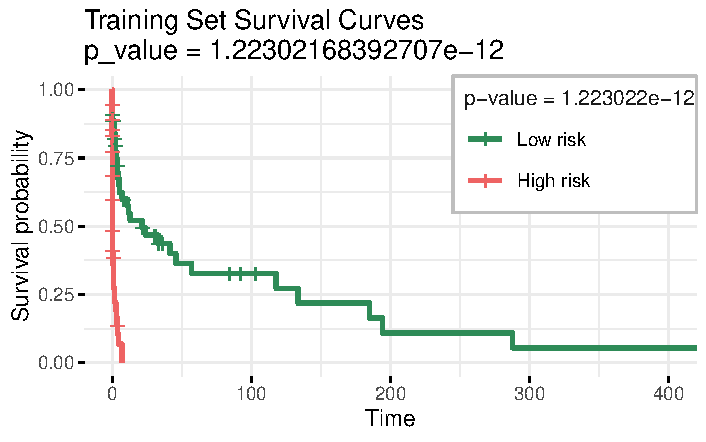
\includegraphics[width=\linewidth]{Fig1_Cox_training_set.pdf}
        %\subcaption{Training set}
        %\label{fig:SURVIVALCURVE_train}
    \end{minipage}
    \begin{minipage}{0.48\linewidth}
        \centering
        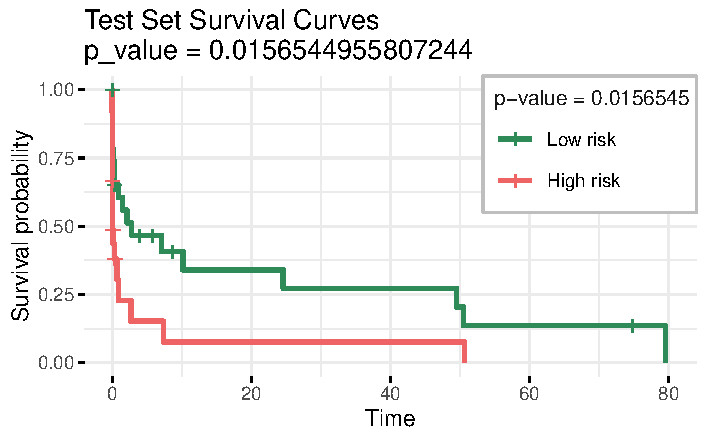
\includegraphics[width=\linewidth]{Fig1_Cox_test_set.pdf}
        %\subcaption{Test set}
        %\label{fig:SURVIVALCURVE_test}
    \end{minipage}
    \caption{The Kaplan-Meier curves in this example are used to visualize and compare survival probabilities, for the train set (left) and for the for test set (right), between two risk groups (High Risk and Low Risk) identified using the Priority Elastic Net Cox proportional hazards model and using function \code{separate2GroupsCox} from \CRANpkg{glmSparseNet} package.}
    \label{fig:SURVIVALCURVE}
\end{figure}

\subsection{Priority-Adaptive elastic net}\label{subsec:PAD-E}

The potential inconsistency of the lasso method in specific scenarios has been explicitly highlighted, as demonstrated by \cite{Zou2005elasticnet}. In response, \cite{Zouadaptivelasso} proposed a modified version of lasso, known as the adaptive lasso and explicitly proved
its consistency in terms of oracle properties asymptotically. Similar ideas are explored in many other papers, namely \citet{zhang2007adaptive} and \citet{wang2007regression}. Apart from
lack of consistency, lasso has other drawbacks as discussed in  \citet{Zou2005elasticnet}, for example, (a) lasso does not encourage grouped selection in case of high pairwise correlation among covariates and (b) for $p>n$ case, lasso can select at most n covariates. To overcome the above drawbacks, they introduced the elastic net, which combines both ridge $\ell_2$ and lasso $\ell_1$ penalties. 
However, the elastic net is not an oracle procedure. Notably, to solve the original elastic net problem \citet{Zou2005elasticnet}, transform the elastic net into an ordinary lasso-type problem
in some augmented space by some algebraic manipulation. Since this is a one-to-one mapping, whenever the lasso is inconsistent in the augmented space, so is the underlying elastic net. For a more detailed discussion on this topic, please refer to \citet{jia2010model}, which states an explicit condition for the inconsistency of the elastic net. Instead of combining the ordinary lasso penalty, the adaptive lasso penalty was integrated with the ridge penalty. This doubly regularised approach, referred to as the adaptive elastic net, aims to leverage the strengths of both penalties.

Another direction for improvement is to correct bias in estimation by adding a weight $w_j$ for each $\beta_j$, corresponding to different amounts of shrinkage, to the regression coefficients.
The adaptive elastic net was introduced by \citet{zou2009adaptive} and \citet{Ghoshadaptiveelastic}, combining the $\ell2$ norm regularisation with adaptive weights to enhance estimation accuracy.

In this context, the elastic net estimates $\hat{\bm{\beta}}_{EN}$ are first computed as defined in \eqref{eq: elastic net}, and then adaptive weights are constructed as follows: 
\begin{equation}
\label{eq:weights}
\hat{w_{j}}=(|\hat{\bm{\beta}}_{EN}|)^{-\gamma}\;\;\;,\;\;\;
 j = 1, 2,  \ldots, p
 \end{equation}
\noindent where $\gamma$ is a positive constant.
Using $\gamma=1$ for calculating adaptive weights in the Adaptive-Elastic net is a common and effective choice because it provides a balance between penalising weak predictors and retaining strong ones.  Since the elastic net naturally adopts a sparse representation, the weights can also be computed a $\hat{w}_j = \left( |\hat{\beta}_{j(\text{EN})}| + \frac{1}{n} \right)^{-\gamma}$ to avoid division by zero \citep{zou2009adaptive}. 
\begin{equation}
\label{eq: adaptive elastic net}
\hat{\bm{\beta}}_{(AENet)} = \arg \min_{\bm{\beta}} \Bigg[ \frac{1}{n}\sum\limits_{i=1}^{n}\bigg(y_i- \beta_{0}- \sum\limits_{j=1}^{p}x_{ij}\beta_j\bigg)^2 +\lambda\sum_{j=1}^p \hat{w_{j}}|\beta{_j}| + \frac{(1 - \alpha)}{2} \sum_{j=1}^{p} \beta_{j}^{2} 
\Bigg].
\end{equation}

Building upon the expression in Equation \eqref{eq: adaptive elastic net}, the framework for the Priority-Adaptive Elastic Net is established by calculating the adaptive weights for the variables based on the assigned priority of the block. Initially, the adaptive weights, denoted as \(\hat{w_j}^{(\bm{\pi})}\) and introduced earlier in \eqref{eq:weights}, are computed for each variable based on the specified priority of the block. In estimating coefficients with the priority-Adaptive Elastic Net, the adaptive weights $\hat{w_j}^{(\pi_1)}$ for the first priority block are incorporated into the $\ell_1$ penalty.

The priority-Adaptive Elastic Net model is formulated by minimising the following objective function for the first block priority:
\begin{equation}
\label{eq:Priority-Elastic}
l(\bm{\beta}^{(\pi_1)}) = \sum_{i=1}^{n}\bigg(y_i - \sum_{j=1}^{p_{\pi_1}}x_{ij}^{(\pi_1)}\beta_j^{(\pi_1)}\bigg)^2 
+ \lambda^{(\pi_1)} \left(\alpha \sum_{j=1}^{p_{\pi_1}} \hat{w_j}^{(\pi_1)}|\beta^{(\pi_1)}_j| 
+ \frac{(1 - \alpha)}{2} \sum_{j=1}^{p_{\pi_1}} \beta_{j}^{2 (\pi_1)} \right).
\end{equation}
Here, the objective function combines a weighted lasso penalty, controlled by $\alpha$ and the adaptive weights $\hat{w_j}^{(\pi_1)}$, with a ridge penalty, balancing sparsity and regularisation.

Using the fitted values from this step as an offset to fit a model considering the covariates in the
block with the second highest priority:
\begin{equation}
\hat{\eta}_{1,i}(\bm{\pi})= \hat{\beta}_1^{(\pi_1)}x_{i1}^{(\pi_1)} + . . . + \hat{\beta}_{p_{\pi_1}}^{(\pi_1)} 
x_{ip_{\pi_1}}^{(\pi_1)}.
\end{equation}

For $b = 2, \dots, B$ (where $B$ is the number of blocks), the model fitting proceeds iteratively. Using the fitted values from Step $b-1$ as an offset, the priority-adaptive elastic net model is then fitted to the covariates in the block with the $b$-th highest priority. 

The implementation of the priority-Adaptive Elastic Net model can be performed using the \CRANpkg{priorityelasticnet} function, as demonstrated in the following code chunk. In this example, the model is applied to Gaussian data with the specified parameters:
{\small
\begin{lstlisting}
fit_gaussian <- priorityelasticnet(
  X = X,  Y = Y,
  family = "gaussian",
  blocks = blocks,
  block1.penalization = TRUE,
  standardize = TRUE,
  lambda.type = "lambda.min",
  max.coef = c(Inf, Inf, Inf),
  nfolds = 10,
  adaptive = TRUE,
  type.measure = "mse",
  initial_global_weight = FALSE,
  alpha = 0.6,
  cvoffset = TRUE,
  cvoffsetnfolds = 10)
\end{lstlisting}
}

In the \code{priorityelasticnet} and \code{cvm\_priorityelasticnet} functions, with the latter presented below, the \code{adaptive} argument controls whether adaptive weights are computed for each block of variables based on their assigned priorities and the estimated coefficient magnitudes. When \code{adaptive = TRUE}, the penalty term becomes data-driven, allowing stronger penalisation of less influential variables and thereby improving variable selection stability and model interpretability. Conversely, when \code{adaptive = FALSE}, all variables within a block are penalised equally, and the model applies fixed, non-data-dependent penalties.

The \code{initial\_global\_weight} argument determines whether global weights across all variables are computed before applying block-specific priorities. Setting 
\code{initial\_global\_weight = TRUE} enables this global assessment step, which is advantageous in most applications because it first derives global weights across all variables and then refines them according to block-specific priorities, capturing both overall and block-level relevance. However, when blocks differ substantially in scale or variability, setting \code{initial\_global\_weight = FALSE} may be preferable, allowing weights to be computed independently within each block and avoiding potential distortion from global weighting. An example of this situation arises when fitting a model that combines clinical, imaging, and genomic data, where it may be important for each block to determine its own internal importance independently of global patterns dominated by larger blocks.

In summary, when both arguments are set to \code{TRUE}, the refinement proceeds in two steps: global adaptive weights are first computed across all variables and are then rescaled according to the block-specific priorities. This two-stage adjustment ensures that both global relevance and block-level importance are reflected in the final regularisation process.

{\small
\begin{lstlisting}
cvm_priorityelasticnet(
  X = matrix(rnorm(100 * 500), 100, 500),
  Y = rnorm(100),
  family = "gaussian",
  alpha = 0.6,
  type.measure = "mse",
  lambda.type = "lambda.min",
  nfolds = 10,
  block1.penalization = TRUE,
  adaptive = TRUE,
  initial_global_weight = FALSE,
  standardize = TRUE,
  cvoffset = TRUE,
  cvoffsetnfolds = 10,
  blocks.list = list(list(bp1 = 1:10, bp2 = 11:30, bp3 = 31:500),
                list(bp1 = 1:10, bp2 = 31:500, bp3 = 11:30)),
  max.coef.list = list(c(Inf, Inf, Inf), c(Inf, 100, Inf)))
\end{lstlisting}
}

After running the function with the specified parameters, the resulting object contains several key outputs, including the best block configuration determined during cross-validation, which differs from the Priority Elastic Net results.

\hypertarget{Summary}{%
\section{Summary}}

Priority Elastic Net is designed to address certain limitations of the Priority-Lasso. Although Priority-Lasso is effective at promoting sparsity, it can perform poorly in the presence of multicollinearity, as it tends to select a single predictor from a set of correlated variables, thereby reducing model stability. The prioritisation framework implemented in Priority Elastic Net allows different block orderings to be evaluated, thereby enabling the contribution of lower-priority predictor groups to be assessed.

The proposed Priority Elastic Net framework \citep{musib2025priorityelasticnet} incorporates the elastic net penalty, balancing $\ell_1$ and $\ell_2$ regularisation. The package also includes the adaptive elastic net formulation that improves variable selection, stable coefficient estimation, and robust performance in high-dimensional, correlated datasets.
Thus, the Priority-adaptive Elastic Net may provide a useful approach for addressing the challenges of modern, complex datasets, with applications in genomics, proteomics, and large-scale predictive modelling. We have thoroughly discussed in \cite{musib2024priority} the advantages of the Priority Elastic Net framework for binary logistic regression. 

The sequential fitting procedure of the \CRANpkg{Priority Elastic Net} can be computationally demanding, particularly when cross-validated offsets are used (\code{cvoffset = TRUE}). Although the current implementation runs sequentially, future versions of the \CRANpkg{priorityelasticnet} package will incorporate parallel execution of cross-validation folds and explore more efficient cross-validation strategies to enhance scalability in high-dimensional, multi-block settings.

In addition, the novel offset imputation strategy, used to enable cross-validation within the sequential block-fitting procedure, may introduce statistical bias that has not yet been formally assessed. As the imputed offsets replace model predictions from higher-priority blocks, any systematic deviation between the imputed and true offsets could propagate through subsequent steps, potentially influencing coefficient estimation or model selection. This aspect will be investigated in future methodological work, both theoretically and through simulation studies. A comprehensive vignette included in the R package provides a detailed walkthrough of the main functions, examples, and use cases, helping users apply the method to their own data.

Further research will also focus on developing simulation studies to systematically compare the predictive accuracy and variable selection stability of the Priority Elastic Net, the Priority Lasso, and the standard Elastic Net across the regression contexts considered in this paper. Real-world applications will also be explored to assess the relative performance of the Priority Elastic Net in practice.

Methodological extensions under consideration include incorporating additional penalisation options, such as SCAD (Smoothly Clipped Absolute Deviation), MCP (Minimax Concave Penalty), and other non-convex penalties, to enhance flexibility and applicability across diverse datasets. These advanced regularisation techniques can mitigate some limitations of convex penalties, offering improved variable selection and estimation in complex scenarios. Finally, extending the package to support multi-response regression models will enable the simultaneous prediction of multiple dependent variables—a valuable feature for applications in genomics, proteomics, and other domains involving high-dimensional, multi-output data. Collectively, these developments aim to broaden the scope and practical utility of the package for researchers working with modern, multifaceted datasets.

\hypertarget{Acknowledgments}{%
\section*{Acknowledgments}}
This work is funded by national funds through FCT – Fundação para a Ciência e a Tecnologia, I.P., under CEAUL Research Unit, UID/00006/2025, DOI: https://doi.org/10.54499/UID/00006/2025, and from the FCT Tenure program, with reference
2023.15441.TENURE.033/CP00003/CT00010.\\

The authors acknowledge the developers of the \CRANpkg{prioritylasso} package \citep{Klau2018prioritylasso,klau2017prioritylasso}, whose implementation served as the basis for several functions included in the \CRANpkg{priorityelasticnet} package.

\bibliography{carrasquinha_etal}

\address{%
Laila Musib\\
Faculdade de Ciências da Universidade de Lisboa \\%
Centro de Estatística e  Aplicações da Universidade de Lisboa (CEAUL)\\%
Campo Grande 016, 1749-016 Lisboa, Portugal\\%
\email{fc59282@alunos.ciencias.ulisboa.pt}
}

\address{%
Helena Mouriño\\
Faculdade de Ciências da Universidade de Lisboa \\%
Centro de Estatística e  Aplicações da Universidade de Lisboa (CEAUL)\\%
Campo Grande 016, 1749-016 Lisboa, Portugal\\%
\email{mhnunes@ciencias.ulisboa.pt}
}

\address{
Eunice Carrasquinha\\
Faculdade de Ciências da Universidade de Lisboa \\%
Centro de Estatística e  Aplicações da Universidade de Lisboa (CEAUL)\\%
Campo Grande 016, 1749-016 Lisboa, Portugal\\%
\email{eitrigueirao@ciencias.ulisboa.pt}
}
